
\subsection{\acfp{TEA}}
\label{section:spectre}
Optimierungsmechanismen, wie Transient Execution und
\ac{OoO}-Execution, können ausgenutzt werden, um auf der \ac{CPU}
Instruktionen auszuführen, die aus architektonischer
Sicht nicht ausgeführt werden sollten.
Dabei kann auf Informationen zugegriffen oder abgeleitet
werden, die für den jeweiligen Prozesskontext nicht
sichtbar sein sollten. (\cite[249,251]{canella_systematic_2019})

Ein Angriff umfasst drei Phasen, die in
Abbildung \ref{figure:transient-attack-phases} dargestellt sind:
Vorbereitung, Ausführung und Auslesen.
In der Vorbereitungsphase wird der Zustand der Mikroarchitektur in
einen gewünschten Zustand versetzt. Beispielsweise werden
Speicheradressen für die Übertragung der Information durch den
\ac{CbCC} evictet oder ein Predictor der \ac{CPU} trainiert.
Danach folgt die Phase der Transient Execution, in der das
gesuchte Secret ausgelesen und in den Covert-Channel geschrieben,
beziehungsweise die Mikroarchitektur verändert wird.
Diese Zustandsänderung kann danach gemessen und daraus die
übertragene Information abgeleitet werden. Das Ende der Transient
Execution führt zum Zurücksetzen des architektonischen Zustands
und das Programm setzt seine normale Ausführung fort. Das
Auslesen des Secrets, beispielsweise aus dem Cache-Zustand,
bringt die Information schließlich in den architektonischen
Zustand des Programms.
(\cite[2]{xiong_survey_2022}, \cite[251]{canella_systematic_2019})

Transient Execution ist dabei nicht garantiert. So können
beispielsweise Branch-In\-struk\-ti\-onen zwischen den Trainingsläufen
den Zustand des Predictors verändern, oder im Falle von dem
ursprünglichen Meltdown Angriff kann die Exception eintreten,
bevor der Wert geladen wurde (\cite[9,10]{lipp_meltdown_2020}).

\begin{figure}
    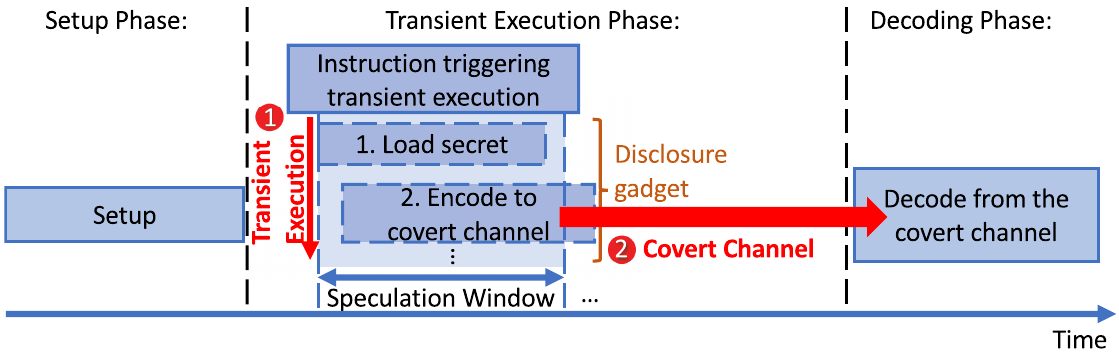
\includegraphics[width=\textwidth]{img/transient-attack-phases.png}
    \caption{Phases of transient execution attacks.
    (\cite[2]{xiong_survey_2022})}
    \label{figure:transient-attack-phases}
\end{figure}

\subsubsection{Einordnung verschiedener Angriffe}
Eine Taxonomie von Angriffen mit Transient Execution wurde von
\cite[252-258]{canella_systematic_2019} vorgeschlagen, ist inzwischen jedoch
teilweise veraltet. Grundsätzlich wird dort zwischen Spectre- und
Meltdown-ähnlichen Angriffen unterschieden. Meltdown-ähn\-liche
Angriffe nutzen \ac{OoO} Execution aus, um Instruktionen, die
auf einen Programmfehler folgen, dennoch auszuführen. Spectre
dagegen nutzt einen Predictor aus, um den Control Flow oder
Datenzugriffe zu manipulieren. Beispiele für in dieser Taxonomie
noch nicht berücksichtigte Angriffe sind solche, die
Load-Adress-Prediction (\cite[9]{kim_slap_2025}) oder
Load-Value-Prediction (\cite[8,9]{kim_flop_2025}) ausnutzen.

Darüber hinaus wird in dieser Einordnung nicht berücksichtigt,
ob der Angreifer die transient
ausgeführten Instruktionen kontrolliert. Ist dies nicht der Fall,
muss die Information - wie bei \cite[8]{kocher_spectre_2019} - über
ein Gadget in den Zustand der Mikroarchitektur geschrieben werden.
Solch ein Gadget ist ein Programmabschnitt in dem Zielkontext,
bei dem der Cache-Zustand abhängig von dem gesuchten Secret
geändert wird. In diesem Falle kann das Auslesen
gewissermaßen als Side-Channel-Angriff betrachtet werden, da
die transient ausgeführten Instruktionen ursprünglich nicht der
Informationsübertragung dienen. Zudem kann die
Art der Encodierung und damit auch die Technik zum Auslesen nur
eingeschränkt gewählt werden. Aus diesem Grund werden Angriffe,
mit Gadgets in dem Zielkontext, in dieser Arbeit nicht weiter
erläutert. Kontrolliert der Angreifer dagegen
die transient ausgeführten Instruktionen, kann er beliebige
Encodierungen und mikroarchitektonische Zustände wählen, wodurch
die Übertragung eher einem Covert-Channel entspricht.

\subsubsection{Zeitlicher Aufwand von \acp{TEA}}
Vollständige Angriffe können wenige Sekunden bis mehrere Stunden
dauern. Dabei werden viele Übertragungen mit den genannten Phasen
ausgeführt, um Speicherbereiche gezielt nach einem Schlüssel zu
durchsuchen (\cite[7-9]{hertogh_rain_nodate}) oder einfach einen
gewissen Speicherbereich zu übertragen (\cite[10]{kim_slap_2025}).
Den größten Zeitaufwand verursachen dabei meistens die Setup-
oder Decode-Phase aus Abbildung \ref{figure:transient-attack-phases}.
Der Grund dafür ist, dass die Transient Execution in der Regel
aus nur wenige Instruktionen besteht und die
Länge des transient Fensters nur grob über die Art der zugrunde
liegenden Abhängigkeit beeinflusst werden kann. Der zeitliche
Aufwand der Setup-Phase hängt dagegen sowohl von der Art der
Transient Execution als auch vom gewählten \ac{CbCC} ab.
Die Dauer der Decode-Phase ist grundsätzlich nur von dem gewählten
\ac{CbCC} abhängig.

Die Art der Transient Execution wird hauptsächlich von der
ausgenutzten Schwachstelle bestimmt und lässt sich größtenteils nur
für spezifische Hardware optimieren. Dies kann beispielsweise durch
die Reduktion der Trainingsläufe auf ein Minimum passieren.
Der \ac{CbCC} hat jedoch, insbesonders bei Meltdown-Angriffen, den
größten Einfluss auf die Gesamtlaufzeit (\cite[10]{lipp_meltdown_2020}).

Wie bereits beschrieben, erfolgt die Übertragung durch \ac{CbCC}
in drei Schritten: Vorbereitung, Encodierung und Auslesen.
Unabhängig davon, in welchem Prozesskontext diese
Phasen ausgeführt werden, findet die Encodierung immer während
der Transient Execution statt, da nur zu diesem Zeitpunkt das
Secret verfügbar ist. Für die zeitliche Optimierung sind daher
insbesondere die Vorbereitung und das Auslesen entscheidend.

Aufgrund der in \ref{section:cbcc-disturbance} beschriebenen
Fehler muss die Übertragung des Secrets mehrfach wiederholt
werden. Zwar besteht grundsätzlich die Möglichkeit
Fehlerkorrekturverfahren in diesem Kontext einzusetzen, dieser
Ansatz wurde jedoch in der mir bekannten Literatur bislang
nicht betrachtet.
Fehlerkorrektur durch Wiederholen des Angriffs und bilden eines
Mittelwerts der Ergebnisse wie in \cite[9]{lipp_meltdown_2020}
verwendet, ist dennoch nötig, da wie beschrieben die Transient
Execution bei \acp{TEA} nicht jedes Mal erfolgreich sein muss und
dies nicht erkannt werden kann.

Zuletzt stellt sich die Frage der Encodierung. Die beiden
möglichen Encodierungen - bitweise oder als Array-Index -
beziehungsweise Kombinationen aus beiden, stellen eine Abwägung
zwischen der Anzahl an Cache-Zustandsänderungen und der
Anzahl übertragener Bits dar.

\subsection{Mitigationen von Spectre und \ac{CbCC}}
Mitigationen gegen \acp{TEA} auf Hardwareebene versuchen
meist Covert-Channels zu verhindern, konzentrieren
sich allerdings nur auf eine spezifische Art von \ac{CbCC},
beispielsweise durch das Verhindern des Ladens von Adressen
während Transient Execution. (\cite[2]{yan_invisispec_2018})
Das Problem dabei ist, dass
potenziell andere Instruktionen, wie \verb|cldemote| in der
Zukunft für die Veränderung des Cache-Zustands verwendet werden
könnten und generell andere Covert-Channels genutzt werden
könnten. (\cite[3,4]{rauscher_systematic_2025})
Die grundlegendste und garantierte Mitigation, wäre das
Entfernen von Transient, und damit \ac{OoO} und spekulativer
Ausführung, aus neuen Prozessoren. Die Folge wäre allerdings eine
deutliche Reduzierung der \ac{CPU}-Performance
(\cite[25]{xiong_survey_2022}), weshalb mir keine in dieser Form
eingesetzten Mitigationen bekannt sind.
Andere Angriffe wurden häufig durch Mikrocode-Updates mitigiert,
wobei diese nicht immer eine vollständige Mitigation garantieren
(\cite[13]{schwarz_zombieload_2019}).
Einige Schwachstellen wurden in dem ausgenutzten Programm für
die spezifisch ausgenutzte Software mitigiert, beispielsweise
durch das Leeren bestimmter Buffer, vor einem Kontextwechsel,
oder erhöhte Speicherisolation.
(\cite[14]{lipp_meltdown_2020}, \cite[13]{schwarz_zombieload_2019})
Das Problem dabei ist, dass auch diese Lösungen zu gewissen
Performanceeinbußen führen. Außerdem besteht das ursprüngliche
Problem weiter, wodurch neue Angriffe auf Basis derselben
Schwachstelle, wie beispielsweise \cite{hertogh_rain_nodate},
entwickelt werden können.
